\documentclass[a4paper, fontsize = 14pt]{article}
\usepackage{hyperref}
\usepackage[warn]{mathtext}
\usepackage[english,russian]{babel}
\usepackage[utf8x]{inputenc} 
 
%математика
\usepackage{subcaption}
\usepackage{eucal}
\usepackage{amsmath,amsfonts,amssymb,amsthm,mathtools}
\usepackage{icomma}
\usepackage{wasysym}
\usepackage{mathrsfs}
 
%оформление текста
\usepackage{setspace}
\onehalfspacing
\usepackage{indentfirst}
\usepackage{scrextend}
 
%геометрия
\usepackage{geometry}
\geometry{left=25mm,right=25mm,
 top=25mm,bottom=30mm}
 
%графика
\usepackage{wrapfig}
\usepackage{graphicx}
\usepackage{pgfplots}
\usepackage{tikz}
\RequirePackage{caption}
\DeclareCaptionLabelSeparator{defffis}{ --- }
\captionsetup{justification=centering,labelsep=defffis}
 
%таблицы
\usepackage{array,tabularx,tabulary,booktabs} 
\usepackage{longtable}  
\usepackage{multirow} 
 
%ссылки
\usepackage{hyperref}
\usepackage{xcolor}
\definecolor{grn}{HTML}{57A14F} %зеленый
\definecolor{rd}{HTML}{E53C44} %красный 
\definecolor{bl}{HTML}{282691} %синий 
\definecolor{bbl}{HTML}{001B6C} %темно-синий
\hypersetup{		
    colorlinks=true,       	
    linkcolor=bbl,          % внутренние ссылки
    citecolor=rd,          % на библиографию
    filecolor=magenta,      % на файлы
    urlcolor=bl           %внешние источники
}
 
% Колонтитулы
\usepackage{fancyhdr} 
 	\pagestyle{fancy}
 	\renewcommand{\headrulewidth}{0.15mm}  
 	\renewcommand{\footrulewidth}{0.15mm}
 	\lfoot{МФТИ, 2021}
 	\rfoot{\thepage}
 	\cfoot{}
 	\rhead{}
 	\chead{}
 	\lhead{}
 
 
\begin{document}

\begin{center} \textbf{
Лабораторная работа №3.6.1Б \\ Спектральный анализ (цифровой осциллограф) \\ 
Мещеряков Всеволод, Б02-001, 26.10.2021}
\end{center} 

\subsection*{Исследование спектра периодической последовательности прямоугольных импульсов}

\begin{figure}[hbt]
	\centering
	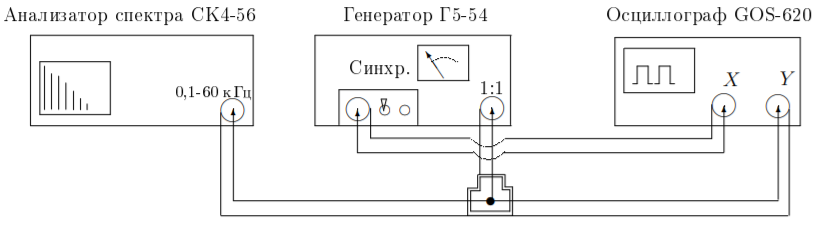
\includegraphics[scale=0.9]{lab361ris1.png}
	\caption{Схема для исследования спектра периодической последовательности прямоугольных импульсов}
\end{figure}

На рисунке 1 представлена схема для исследования спектра периодической последовательности прямоугольных импульсов. Сигнал с выхода генератора прямоугольных импульсов Г5-54 подаётся на вход анализатора спектра и одновременно на вход Y осциллографа. С генератора импульсов на осциллограф также подаётся сигнал синхронизации, запускающий ждущую развертку осциллографа. При этом на экране осциллографа можно наблюдать саму последовательность прямоугольных импульсов, а на экране анализатора спектра -- распределение амплитуд спектральных составляющих этой последовательности.

В наблюдаемом спектре отсутствует информация об амплитуде нулевой гармоники, т.е. о величине постоянной составляющей; её положение (начало отсчёта шкалы частот) отмечено небольшим вертикальным выбросом.

Установим на анализаторе спектра режим работы с однократной разверткой и получим на экране спектр импульсов с параметрами $f_{повт} = 10^3 Гц; \tau = 25 мкс;$ частотный масштаб $m_x = 5кГц/дел$. Проведем измерения зависимости ширины спектра от длительности импульса $\Delta \nu(\tau)$ при увеличении $\tau$ от 25 до 200 мкс. Результаты занесем в таблицу 1.


\begin{table}[hbt]
\centering
\begin{tabular}{|c|c|}
\hline
\textbf{$1/ \tau, 10^{-3} с$} & \textbf{$\Delta \nu(\tau), кГц$} \\ \hline
40                            & 36                               \\ \hline
20                            & 18,5                             \\ \hline
13,3                          & 12                               \\ \hline
10                            & 10                               \\ \hline
8                             & 8                                \\ \hline
6,7                           & 7                                \\ \hline
5,7                           & 6                                \\ \hline
\end{tabular}
\caption{Результаты измерения после пересчёта в единицы измерения, $m_x = 5 кГц/дел$}
\end{table}

Видно, что соотношение неопределенности $\Delta \nu(\tau) \tau = 1$ выполняется с большой точностью и правая часть равна $0,98 \pm 0,06$.

\begin{figure}[hbt]
	\centering
	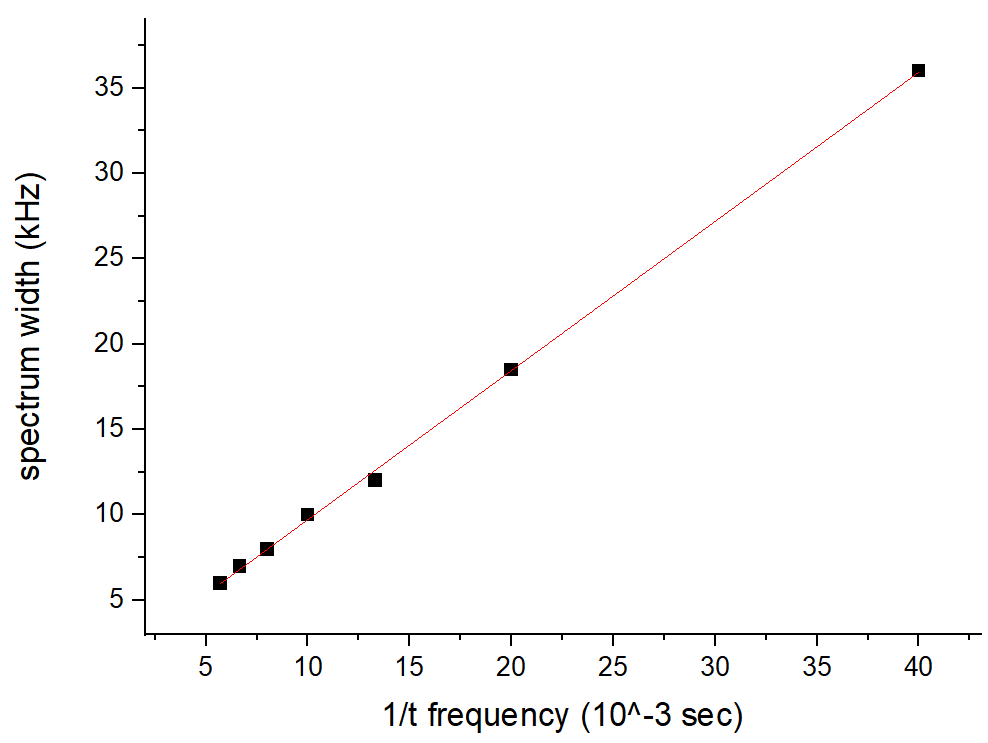
\includegraphics[scale=0.5]{lab361ris2.png}
	\caption{График снятой зависимости $\Delta \nu(1 / \tau)$}
\end{figure}

\newpage

\subsection*{Исследование спектра периодической последовательности цугов гармонических колебаний}

\begin{figure}[hbt]
	\centering
	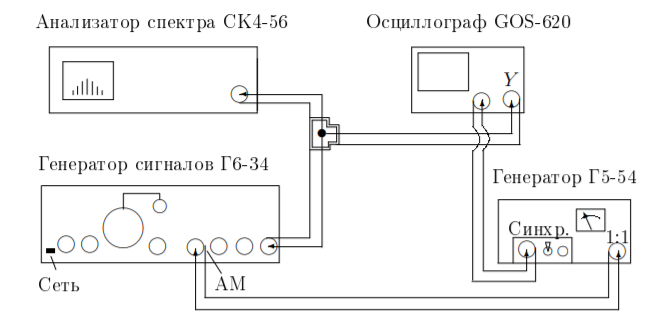
\includegraphics[scale=0.8]{lab361ris8.png}
	\caption{Схема для исследования спектра периодической последовательности цугов гармонических колебаний}
\end{figure}

Установим частоту несущей $\nu_0 = 25 кГц$. Посмотрим, как меняется вид спектра при увеличении длительности вдвое -- рисунок 3. Видно, что с увеличением длительности импульса в два раза ширина спектра уменьшается в два раза, а амплитуды гармоник возрастают в два раза.

\begin{figure}[hbt]
\centering
\begin{tabular}{cc}
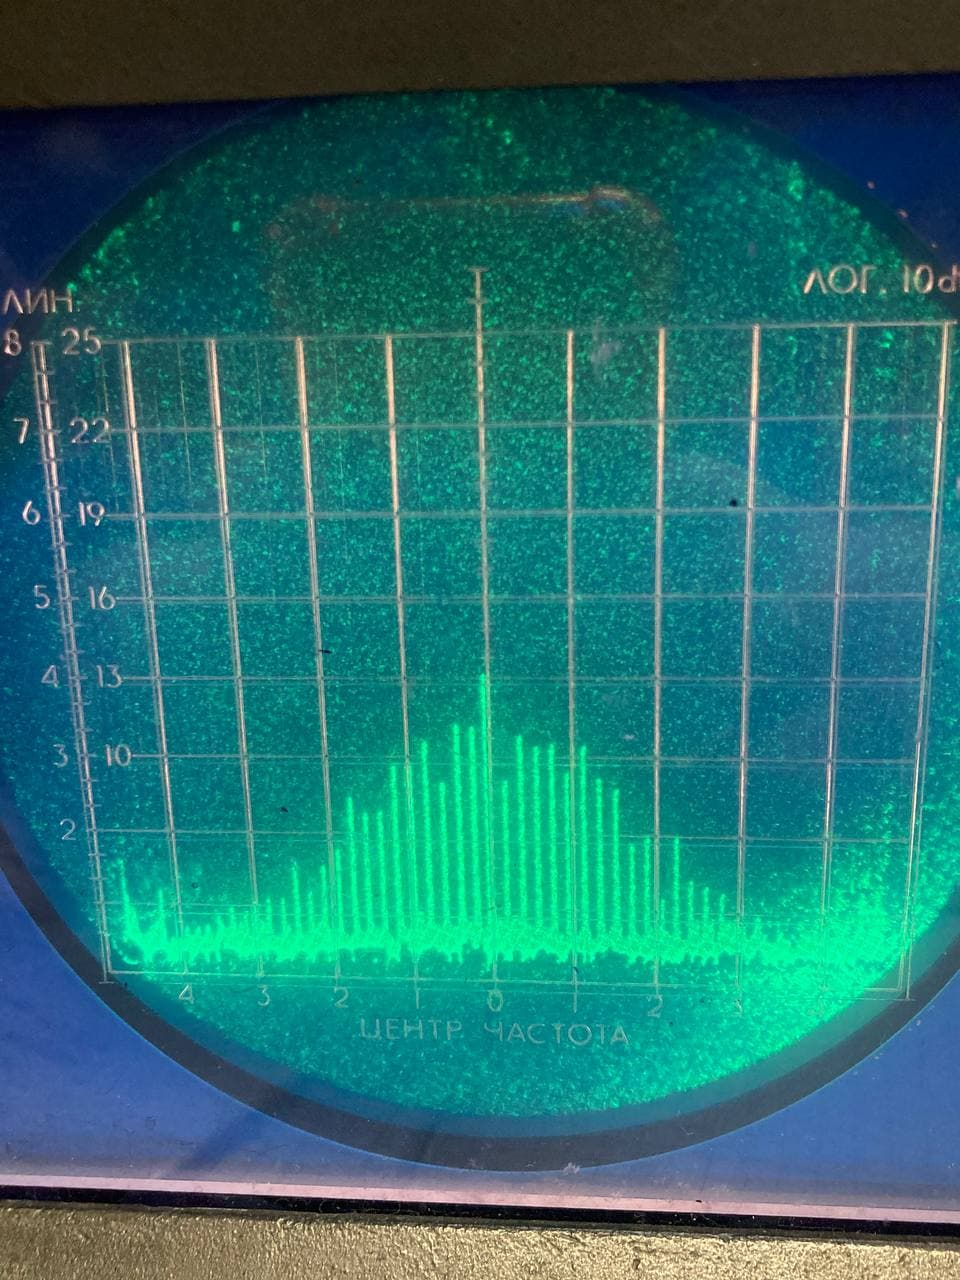
\includegraphics[scale=0.3]{lab361ris3.png}
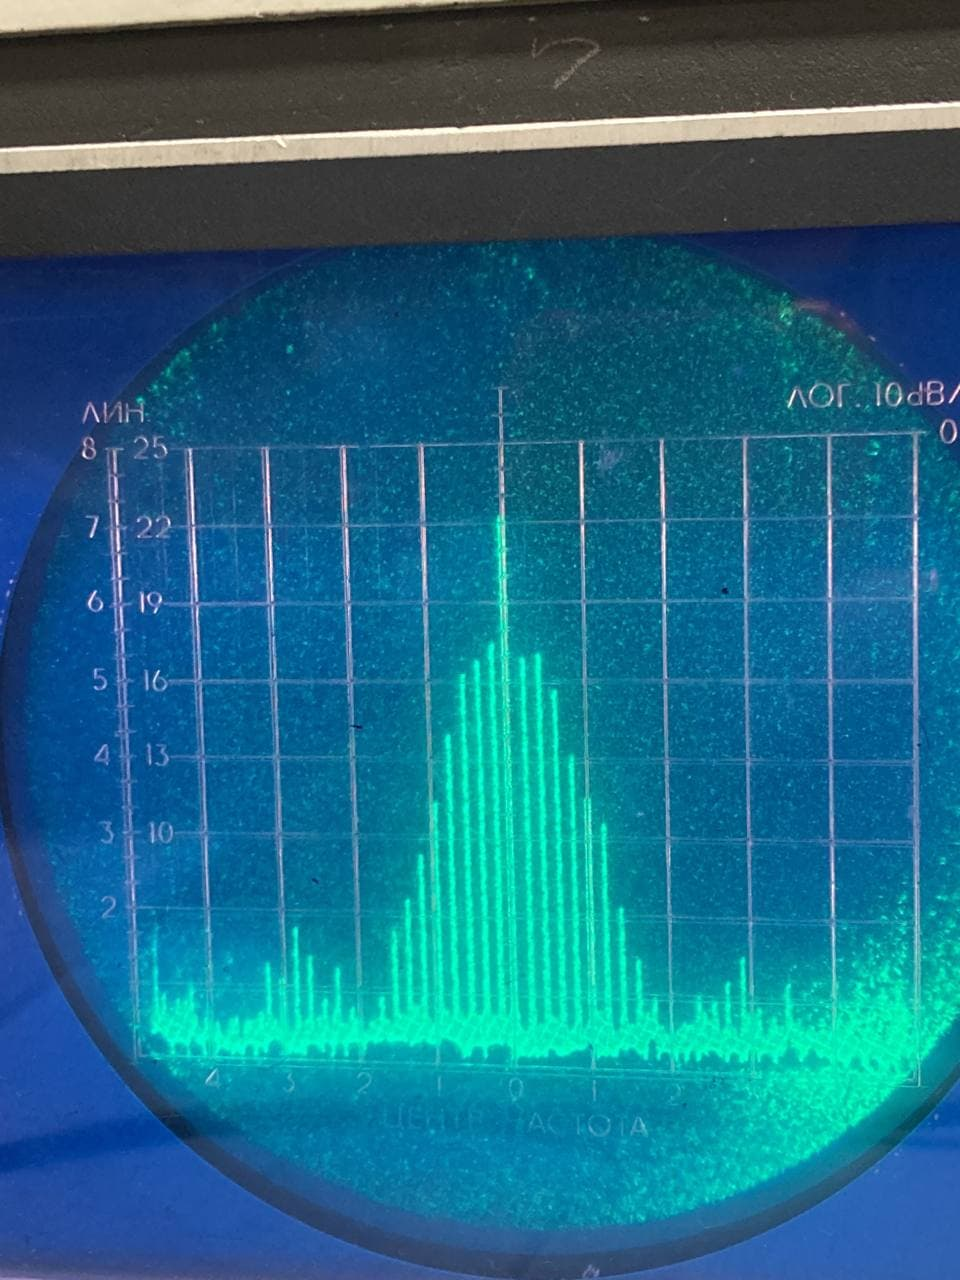
\includegraphics[scale=0.3]{lab361ris4.png}
\end{tabular}
\caption{Спектры при длительности импульса 50мкс (левая фотография), 100мкс (правая фотография)}
\end{figure}

\newpage

Теперь будем изменять несущую частоту $\nu_0$ при фиксированных значениях $f_{повт} = 1 кГц, \tau = 100 мкс$ и частотном масштабе $m_x = 5 кГц/дел$. Видно, что при её увеличении пик сдвигается от начала отсчёта вправо. Для нас это значит, что колебания проходят с теми же амплитудами, но уже на бОльших частотах (гармониках).

\begin{figure}[hbt]
\centering
\begin{tabular}{cc}
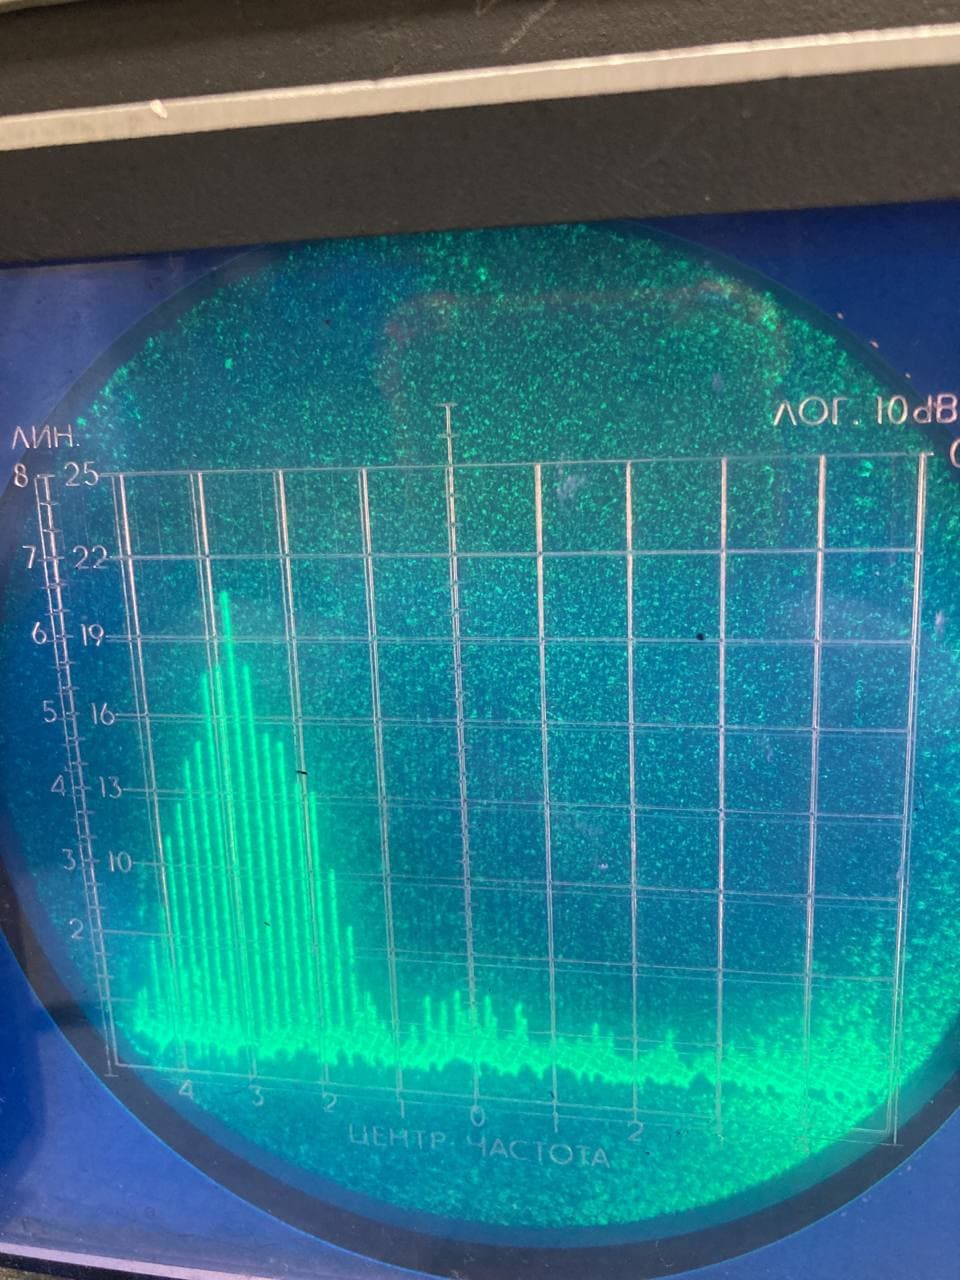
\includegraphics[scale=0.25]{lab361ris5.png}
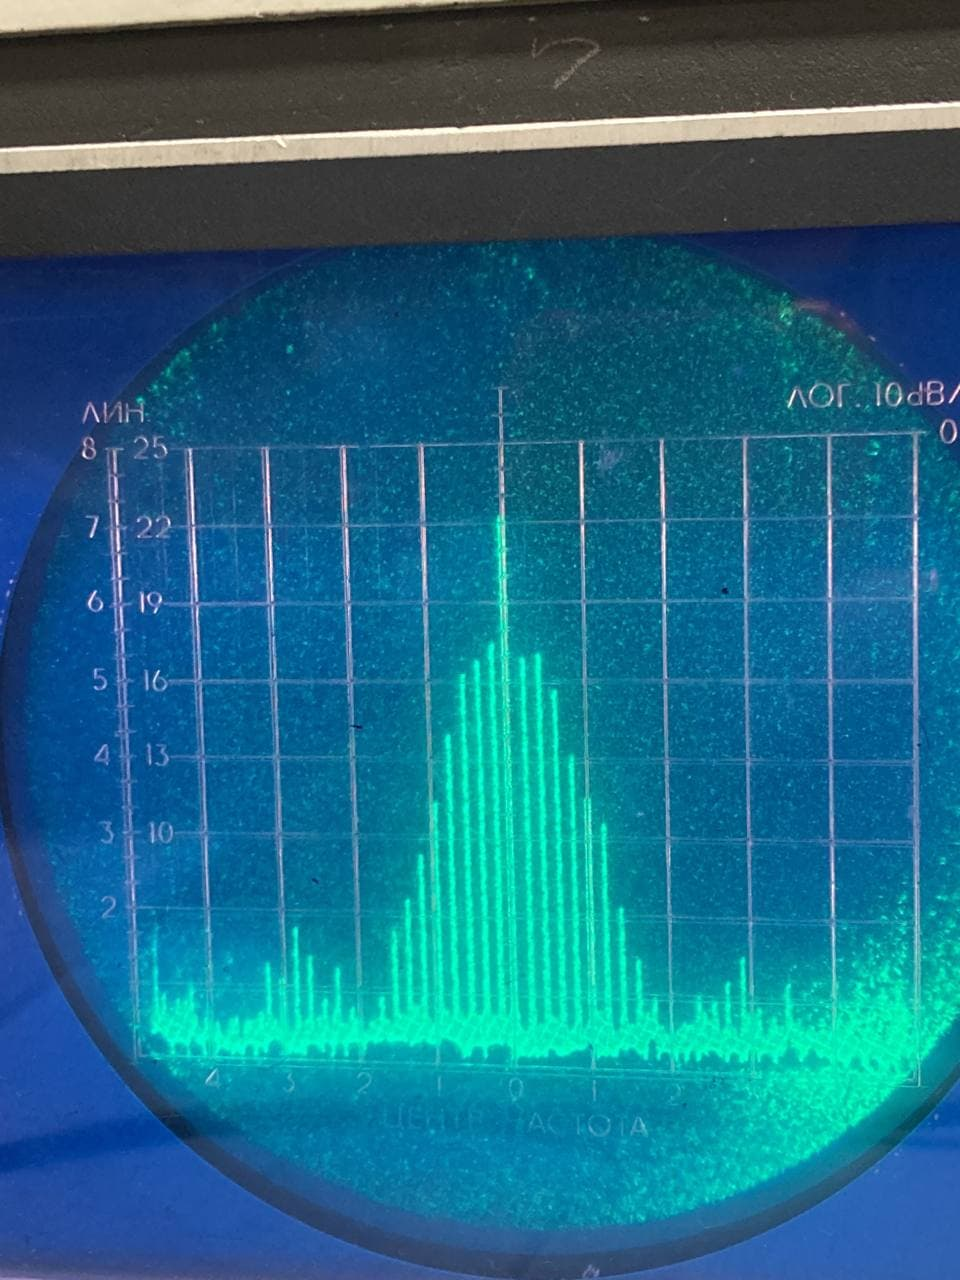
\includegraphics[scale=0.25]{lab361ris6.png}
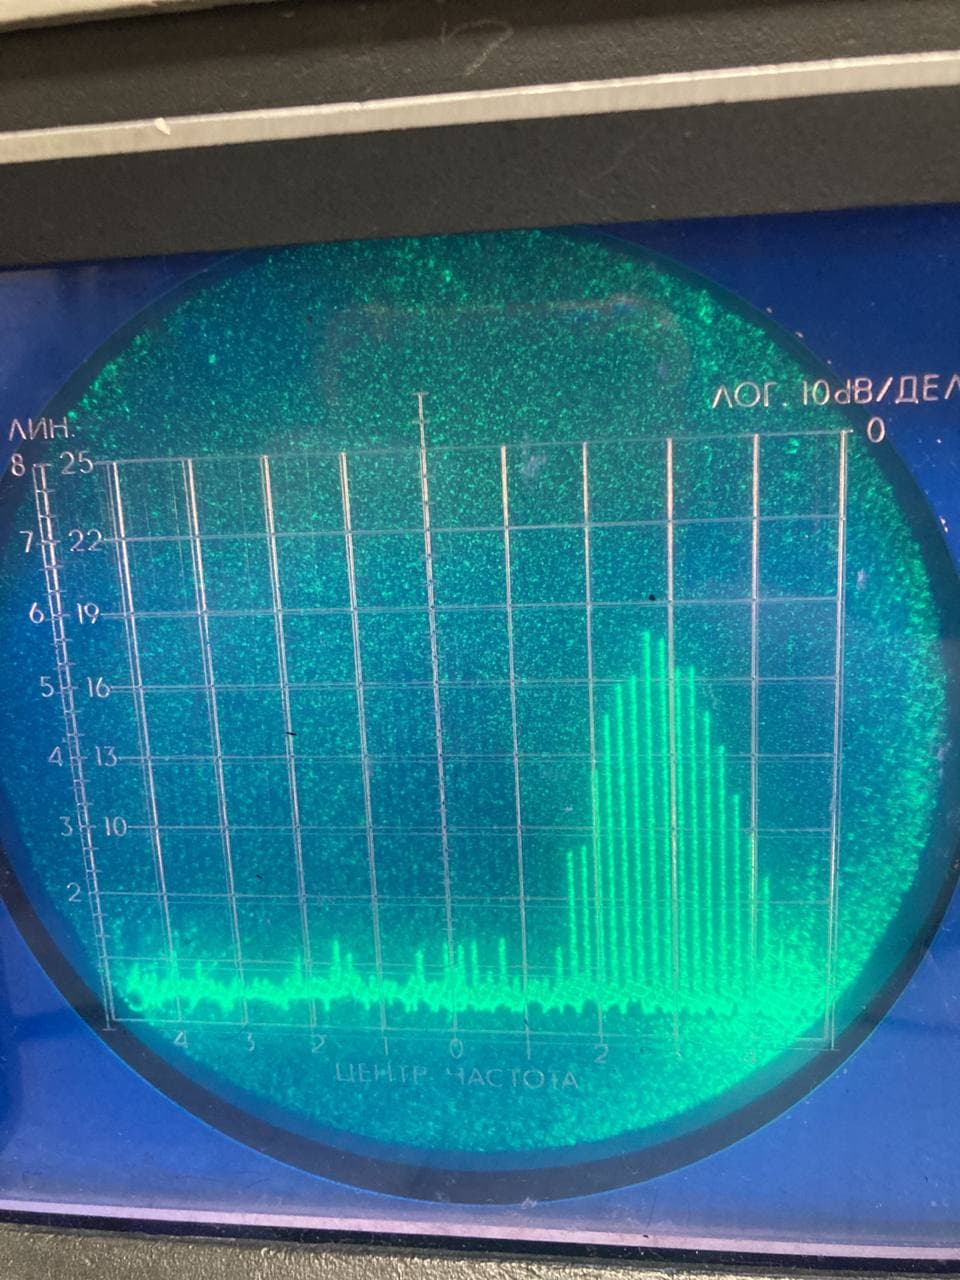
\includegraphics[scale=0.25]{lab361ris7.png}
\end{tabular}
\caption{Спектры при несущей частоте $\nu_0$ 10 кГц (слева), 25 кГц (по центру), 40 кГц (справа)}
\end{figure}

Зафиксируем длительность импульсов $\tau = 50 мкс$ и изучим зависимость $\delta \nu$ меэжу соседними спектральными компонентами от периода $T ( частоты \, повтореняия \, f_{повт}$ в диапазоне 1-8 кГц, подбирая удобный для измерения горизонтальный масштаб $m_x$. Результаты измерений нанесем на плоскость и получим график зависимости $\delta \nu (f_{повт})$ -- рисунок 6.

\begin{figure}[hbt]
	\centering
	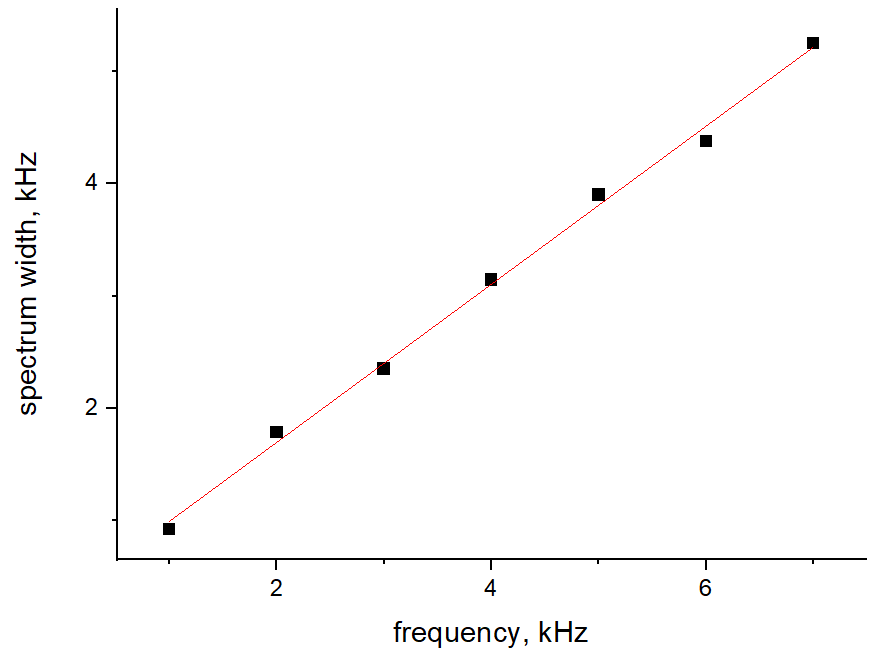
\includegraphics[scale=0.4]{lab361ris9.png}
	\caption{$\delta \nu (f_{повт})$}
\end{figure} 

\newpage

\subsection*{Исследование спектра гармонических сигналов, модулированных по амплитуде}

\begin{figure}[hbt]
	\centering
	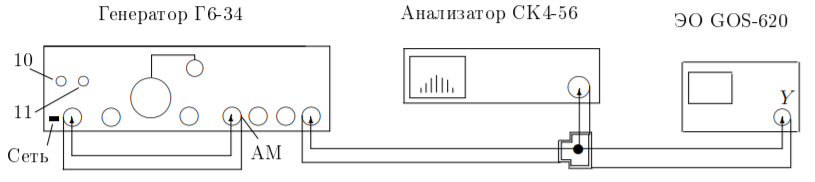
\includegraphics[scale=0.8]{lab361ris10.png}
	\caption{Схема установки для исследования спектра гармонических сигналов, модулированных по амплитуде}
\end{figure}

Будем изменять глубину модуляции и снимать зависимость отношения амплитуды боковой линии спектра к амплитуде основной линии $(a_{бок}/a_{осн})$. На рисунке 8 отразим полученную зависимость. Из графика получаем угол наклона прямой f(m) равным $0,58 \pm 0,05$.

\begin{figure}[hbt]
	\centering
	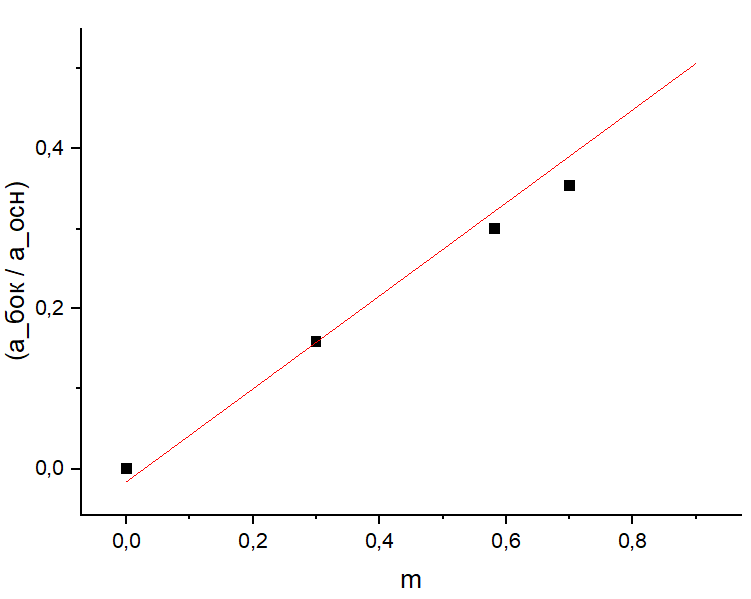
\includegraphics[scale=0.6]{lab361ris11.png}
	\caption{График зависимости $\frac{a_{бок}}{a_{осн}}(m)$}
\end{figure}

Выставим глубину модуляции нулевой (m = 0) и посмотрим, как меняется спектр при увеличении частоты модулирующего сигнала. На качественном уровне происходит расширение спектра, количество и высота гармоник остаются прежними. Боковые пики отдаляются от основного, который стоит на месте.
\end{document}